\section{Data processing}
\label{s:DataGAProcessing}

One of the components developed in this research is the \textsc{packet capture parser}, further described in section \ref{ss:PcapParser}.
Inputs to this parser are the result directory containing packet captures captured by each worker during each separate scan task and also an IP ignore list to filter out unwanted IP addresses. The retrieval component synchronizes packet captures to an output directory given by an input parameter. To separate each task from the other for use in the analysis, the directory tree structure for the retrieved packet capture is shown in figure \ref{fig:LabTree}.

\begin{figure}[htbp]
\centerline{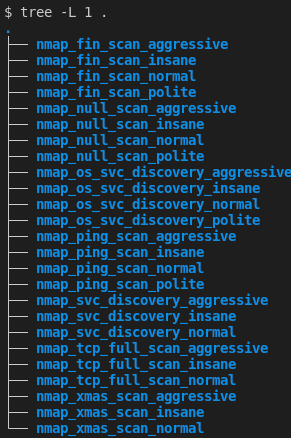
\includegraphics[scale=0.50]{images/lab/treepcap.png}}
\caption{Capture of tree directory structure for retrieved packet captures.}
\label{fig:LabTree}
\end{figure}

The parser then iterates through the given result directory identifying each respective task by name and the respective files related to the task. Scapy is used to read each representative packet captured into an object. Furthermore, header fields are defined for IP, TCP, UDP, and ICMP header, which are directly written to a file, each resulting in 3 files (TCP, UDP, and ICMP), with the pattern enlisted as \textit{protocol\_taskname\_scannumber\_timestamp.csv}.
Each packet is iterated through, where only IP packets are processed. The parser creates a list of each packet during the iteration and detects the protocol before writing the packet details into its representative CSV file.
Another Python library used during iteration is the binascii library, which decodes the payload to hex.
A comparison of the raw packet capture and the parsed CSV file is shown in figure \ref{fig:LabPacketCSV}.
Within the figure, the top 5 lines, including the read message in tcpdump of the raw packet capture file, and the top 5 lines, including the header of the CSV file, are shown as a comparison of the formats.
Colorized in the figure are corresponding services in the packet capture file with the port number outlined in the CSV file.
As we can see, the telnet service is outputted in the CSV file as port 23, enlisted with the green color.



\begin{figure}[htbp]
\centerline{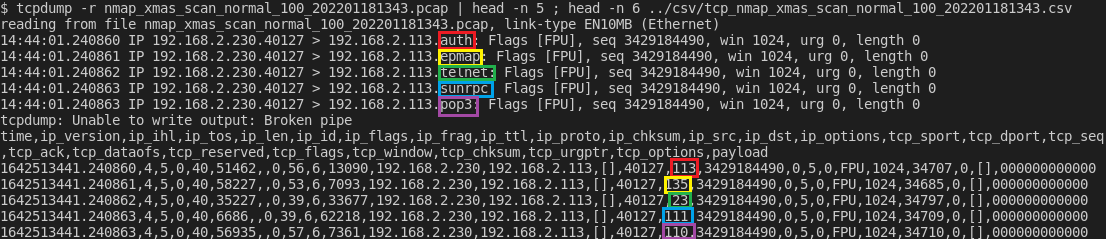
\includegraphics[scale=0.4]{images/lab/tcpdumpcsvdiff.png}}
\caption{Capture of comparison of raw packet capture and parsed CSV output.}
\label{fig:LabPacketCSV}
\end{figure}

%% ---------------------------- PCAP PARSER ----------------------------
\subsection{Packet capture parser}
\label{ss:PcapParser}

A packet capture parser was needed for parsing raw packet capture files into comma-separated value (CSV) files.
This format is easier to work with and extract data later in the process.
The parser is written in Python and uses one user input argument for setting the path for the given packet capture file that is going to be parsed.

\subsubsection{Python libraries}
Python libraries used in the parser are CSV, sys, os, binascii, and scapy.

The \textit{csv} library are used for writing to CSV files. \textit{sys} is used for exiting the parser and capturing the given input when executing the parser. The os library is used for retrieving the directory and basename for the given packet capture file.
Within the binascii library, the hexlify function is used for decoding TCP and UDP payloads to hex format.
Scapy\footnote{https://scapy.net/} are the key library used for the parser. Scapy is used to read the packet capture and extract all relevant content.
The choice for using Scapy is based on personal preferences and familiarisation during earlier projects such as the FenrisBox, where Scapy was used to modify packets \autocite{Jacobsen_FenrisBox_2021}.

Within listing \ref{lst:CSVHeaderPcapParser} a header structure for CSV files are generated.
The output after running this code is three CSV files, each file containing the given protocol.
The write operation is defined within lines 1 to 6, and the operation itself is executed in lines 14, 17, and 22 in listing \ref{lst:CSVHeaderPcapParser}. Usage of the same writing operations is done later in the parser also.

The parser writes to three different files, each identified by the protocol in the name. This will return a file multiplication of three files for each packet capture file processed.


\begin{listing}[!ht]
\caption{Generating CSV header in the Pcap Parser}
\label{lst:CSVHeaderPcapParser}
\begin{minted}[linenos]{Python}
output_tcp = csv.writer(open(dir_name + '/output_tcp_' + base_name.replace(".pcap","") +
'.csv', 'w'), delimiter=',', quotechar='"', quoting=csv.QUOTE_MINIMAL)
output_udp = csv.writer(open(dir_name + '/output_udp_' + base_name.replace(".pcap","") + 
'.csv', 'w'), delimiter=',', quotechar='"', quoting=csv.QUOTE_MINIMAL)
output_icmp = csv.writer(open(dir_name + '/output_icmp_' + base_name.replace(".pcap","") + 
'.csv', 'w'), delimiter=',', quotechar='"', quoting=csv.QUOTE_MINIMAL)

ip_header = ['time', 'ip_version', 'ip_ihl', 'ip_tos', 'ip_len', 'ip_id', 'ip_flags', 
'ip_frag', 'ip_ttl', 'ip_proto', 'ip_chksum', 'ip_src', 'ip_dst', 'ip_options']

ip_tcp_header = (ip_header + ['tcp_sport', 'tcp_dport', 'tcp_seq', 'tcp_ack', 'tcp_dataofs', 
'tcp_reserved', 'tcp_flags', 'tcp_window', 'tcp_chksum', 'tcp_urgptr', 'tcp_options', 
'payload'])
output_tcp.writerow(ip_tcp_header)

ip_udp_header = (ip_header + ['udp_sport', 'udp_dport', 'udp_len', 'udp_chksum', 'payload'])
output_udp.writerow(ip_udp_header)

ip_icmp_header = (ip_header + ['icmp_type', 'icmp_code', 'icmp_chksum', 'icmp_id', 
'icmp_seq', 'icmp_ts_ori', 'icmp_ts_rx', 'icmp_gw', 'icmp_ptr', 'icmp_reserved', 
'icmp_length', 'icmp_addr_mask', 'icmp_nexthopmtu', 'icmp_unused', 'payload'])
output_icmp.writerow(ip_icmp_header)
\end{minted}
\end{listing}

The parser extracts IP header values as a bare minimum, shown in figure \ref{fig:IPHeader}.

The values within the IP header in figure \ref{fig:IPHeader} is paired against the fields defined in lines 8 and 9 in listing \ref{lst:CSVHeaderPcapParser} and the values used in Scapy.
This pairing is documented in table \ref{tbl:IPScapySimilarities}.

\begin{figure}[ht]%
    \centering
    \subfloat[IP header\label{fig:IPHeader}]{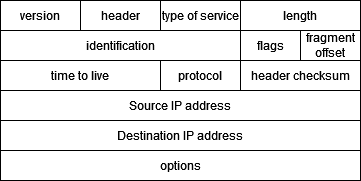
\includegraphics[scale=0.6]{images/misc/IP-header.png}}
    \qquad
    \subfloat[TCP header\label{fig:TCPHeader}]{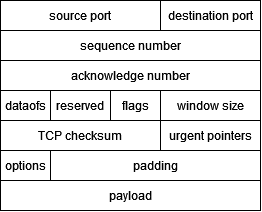
\includegraphics[scale=0.6]{images/misc/TCP-header.png}}\\
    \subfloat[UDP header\label{fig:UDPHeader}]{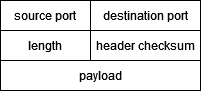
\includegraphics[scale=0.6]{images/misc/UDP-header.png}}
    \qquad
    \subfloat[ICMP header\label{fig:ICMPHeader}]{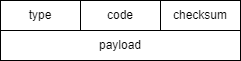
\includegraphics[scale=0.6]{images/misc/ICMP-header.png}}
    \caption{IP, TCP, UDP and ICMP header}
    \label{fig:Headers}%
\end{figure}




\begin{table}[htbp]
\caption{Mapping between CSV fields, IP/TCP/UDP/ICMP header and Scapy}
\begin{center}
%\begin{tabular}{|c|c|c|c|c|c|c|}
\begin{tabular}{|l|l|l|l|l|l|l|}
\hline
IP header               & CSV                   & Scapy && TCP header & CSV & Scapy\\
\hline
Version                 & \textit{ip\_version}  & \textit{version}&& Source port & \textit{tcp\_sport} & \textit{sport}\\
\hline
Header                  & \textit{ip\_ihl}      & \textit{ihl}&&Destination port & \textit{tcp\_dport} & \textit{dport}\\
\hline
Type of service         & \textit{ip\_tos}      & \textit{tos}&& Sequence number & \textit{tcp\_seq} & \textit{seq}\\
\hline
Length                  & \textit{ip\_len}      & \textit{len}&& Acknowledge number & \textit{tcp\_ack} & \textit{ack}\\
\hline
Identification          & \textit{ip\_id}       & \textit{id}&& Dataofs & \textit{tcp\_dataofs} & \textit{dataofs}\\
\hline
Flags                   & \textit{ip\_flags}    &\textit{flags}&& Reserved & \textit{tcp\_reserved} & \textit{reserved}\\
\hline
Fragment offset         & \textit{ip\_frag}     &\textit{frag}&& Flags & \textit{tcp\_flags} & \textit{flags}\\
\hline
Time to live            & \textit{ip\_ttl}      &\textit{ttl}&& Window size & \textit{tcp\_window} & \textit{window}\\
\hline
Protocol                & \textit{ip\_proto}    &\textit{proto}&& TCP checksum & \textit{tcp\_chksum} & \textit{chksum}\\
\hline
Header checksum         & \textit{ip\_chksum}   &\textit{chksum}&& Urgent pointers & \textit{tcp\_urgptr} & \textit{urgptr}\\
\hline
Source IP               & \textit{ip\_src}      &\textit{src}&& Options & \textit{tcp\_options} & \textit{options}\\
\hline
Destination IP          & \textit{ip\_dst}      &\textit{dst}&& Payload & \textit{payload} & \textit{payload}\\
\hline
Options                 & \textit{ip\_options}  &\textit{options}&& & & \\
\hline
\multicolumn{7}{|c|}{ }\\
\hline
UDP header & CSV & Scapy &&  ICMP header & CSV & Scapy\\
\hline
Source port & \textit{udp\_sport}&\textit{sport}&& Type & \textit{icmp\_type} & \textit{type}\\
\hline
Destination port & \textit{udp\_dport}&\textit{dport}&& Code & \textit{icmp\_code} & \textit{code}\\
\hline
Length & \textit{udp\_len}&\textit{len}&& Checksum & \textit{icmp\_chksum} & \textit{chksum}\\
\hline
Checksum & \textit{udp\_chksum}&\textit{chksum}&& ID & \textit{icmp\_id} & \textit{id}\\
\hline
Payload & \textit{payload}&\textit{payload}&& Sequence number & \textit{icmp\_seq} & \textit{seq}\\
\hline
& &&& Originate timestamp & \textit{icmp\_ts\_ori} & \textit{ts\_ori}\\
\hline
& &&& Receive timestamp & \textit{icmp\_ts\_rx} & \textit{ts\_rx}\\
\hline
& &&& Gateway & \textit{icmp\_gw} & \textit{gw}\\
\hline
& &&& Pointer  & \textit{icmp\_ptr} & \textit{ptr}\\
\hline
& &&& Reserved & \textit{icmp\_reserved} & \textit{reserved}\\
\hline
& &&& Length & \textit{icmp\_length} & \textit{length}\\
\hline
& &&& Addr mask & \textit{icmp\_addr\_mask} & \textit{addr\_mask}\\
\hline
& &&& Next-hop MTU & \textit{icmp\_nexthopmtu} & \textit{nexthopmtu}\\
\hline
& &&& Unused & \textit{icmp\_unused} & \textit{unused}\\
\hline
& &&& Payload & \textit{payload} & \textit{payload}\\
\hline
\end{tabular}
\label{tbl:IPScapySimilarities}
\end{center}
\end{table}


Depending on which protocol each packet is identified with, the parser is able to extract values from the TCP header (shown in figure \ref{fig:TCPHeader}), UDP header (shown in figure \ref{fig:UDPHeader}), and ICMP header (shown in figure \ref{fig:ICMPHeader}).

The ICMP header is different from the TCP and UDP header, which have fixed fields.
There are 3 fixed values for the ICMP header, which are type, code, and checksum.
Remaining of the ICMP header depends on the \textit{type} given according to RFC 792 \autocite{rfc792}.
This meaning, if the ICMP code is either $8$ (echo message) or $0$ (echo reply message) the ICMP header would include the \textit{identifier} and \textit{sequence number} fields as visualised in figure \ref{fig:ICMPEchoHeader}.
As seen in these figures and table \ref{tbl:IPScapySimilarities}, Scapy is able to extract all the values for a packet.


\begin{figure}[ht]%
    \centering
    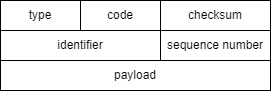
\includegraphics[scale=0.6]{images/misc/ICMP-Echo-Header.png}
    \caption{ICMP echo header}
    \label{fig:ICMPEchoHeader}%
\end{figure}

\newpage



\newpage

\subsection{Bulk pcap parser}
This script has the objective of iterating through a given directory containing packet capture files.
Inputs to the script is the path to the directory where the \textsc{packet capture parser} is located and the location of the directory containing the packet capture files to be parsed.
It identifies each packet capture file within a given directory and executes the \textsc{packet capture parser}.

\begin{listing}[!ht]
\caption{Execute bulk pcap parsing using Python Pcap parser}
\label{lst:BulkPcapParser}
\begin{minted}{Bash}
#!/bin/bash
# Parse PCAP to CSV
PARSER_PATH=$1
PCAP_DIR=$2

if [ -z $PCAP_DIR ] && [ -z $PARSER_PATH ]; then
  echo "usage: bash $0 <path to pcap parser> <pcap directory>";
  exit
fi

for FILE in $(find $PCAP_DIR -name "*cap" -type f); do
  FILENAME=$(basename $FILE)
  DIRNAME=$(dirname $FILE)

  python3 $PARSER_PATH/pcap_argv_parser.py $FILE
done
\end{minted}
\end{listing}
%% ---------------------------- /PCAP PARSER ----------------------------


